\chapter{Grundlagen des Spiels Vier Gewinnt}

\section{Spielregeln und Spielablauf}
%Die Regeln für dieses Strategiespiel sind kinderleicht, was auch ein Argument für die große Beliebtheit bei Jung und Alt ist. Das Spiel besteht aus einem senkrecht stehenden Spielbrett und jeweils aus 21 gelben und roten runde Steine. Diese Steine werden abwechselnd in das hohle Spielbrett mit 42 Aussparungen, sieben Spalten und sechs Reihen, eingeworfen. Der Spieler kann somit eine Spalte auswählen und den Stein fallen lassen. Der eingeworfene Stein besetzt den untersten freien Platz dieser Spalte. Das Spiel wird dann gewonnen, wenn einer der Spieler vier oder mehr Steine in einer waagerechten, senkrechten oder diagonalen Reihe platzieren kann. Der andere Spieler hat somit automatisch verloren. Kommt es zu keiner Bildung einer dieser Kombinationen, endet das Spiel bei Vergabe aller Steine in einem Remis.

Das originale Spiel 4Gewinnt besteht aus einer Rasterwand mit sechs Zeilen und sieben Spalten, also 42 Löchern. Außerdem besteht es aus 21 roten Spielchips und 21 gelben Spielchips. 4Gewinnt lässt sich nur zu zweit spielen. Ziel des Spieles ist es, vier Spielchips einer Farbe in eine Reihe (waagrecht, senkrecht oder diagonal) zu bringen. Der jüngste Spieler beginnt das Spiel. Der Spieler, der an der Reihe ist, wirft einen Spielstein seiner Farbe durch die Öffnung der Rasterwand, wo durch der gespielte Stein auf den untersten freien Platz in der Spalte fällt. Danach ist der andere Spieler an der Reihe. Die Spieler werfen so lange ihre Spielchips in das Raster, bis einer das Ziel erreicht hat oder alle 42 Felder belegt sind. Für den Fall, dass alle 42 Felder des Rasters belegt sind, endet das Spiel unentschieden. Um ein neues Spiel zu starten, muss ein Spieler die Steine aus dem Raster fallen lassen. Diese werden dann wieder unter den Spielern aufgeteilt und eine neue Runde 4Gewinnt kann beginnen\autocite{Hasbro.2020}.

\begin{figure}[H]
	\centering
	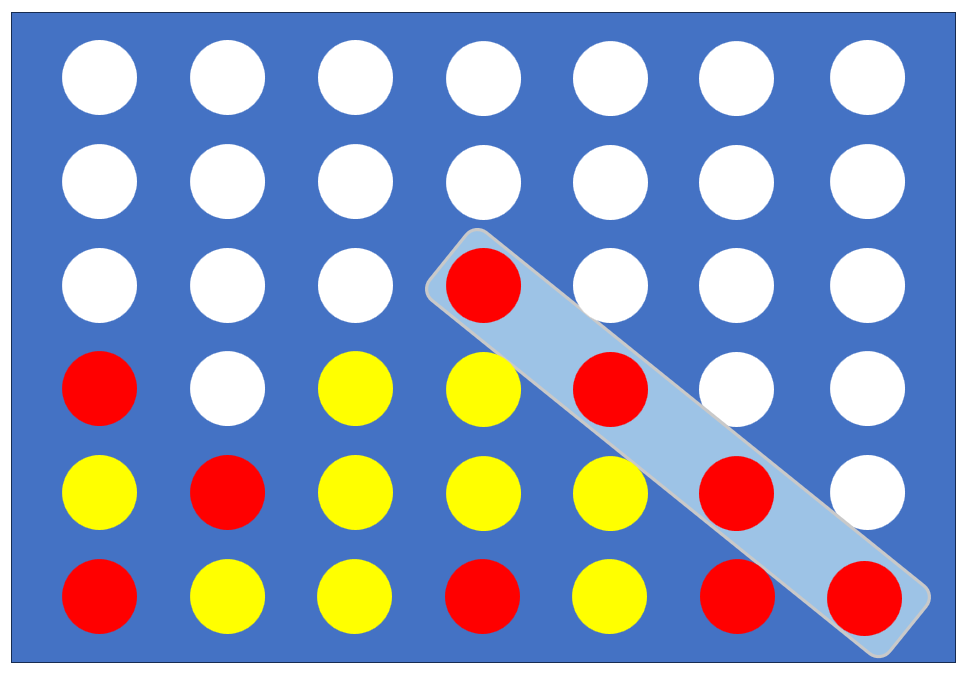
\includegraphics[width=0.8\linewidth]{images/Diagonal}
	\caption[Vier rote Steine diagonal]{Vier rote Steine diagonal im Raster}
	\label{fig:diagonal}
\end{figure}
\begin{figure}[H]
	\centering
	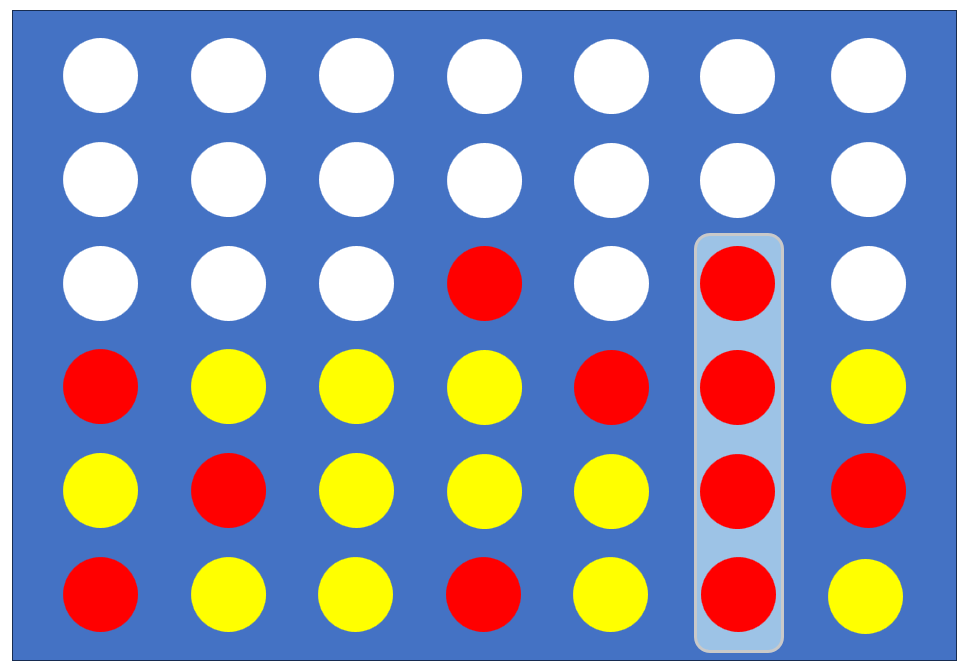
\includegraphics[width=0.8\linewidth]{images/Senkrecht}
	\caption[Vier rote Steine in Reihe senkrecht]{Vier rote Steine senkrecht im Raster}
	\label{fig:senkrecht}
\end{figure}
\begin{figure}[H]
	\centering
	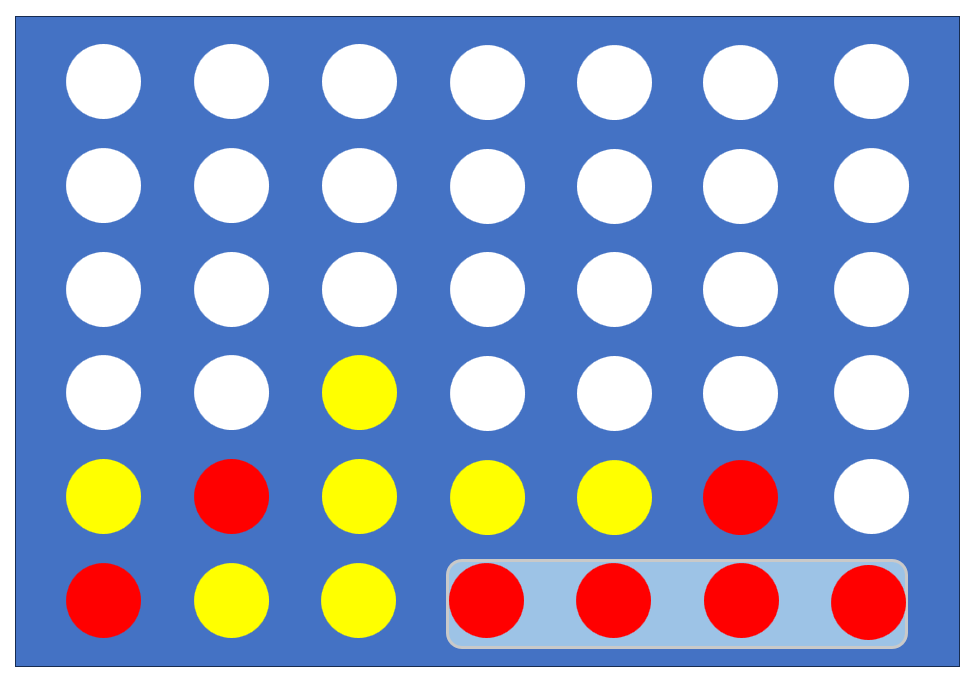
\includegraphics[width=0.8\linewidth]{images/Waagrecht}
	\caption[Vier rote Steine in Reihe waagrecht]{Vier rote Steine waagrecht im Raster}
	\label{fig:waagrecht}
\end{figure}
\begin{figure}[H]
	\centering
	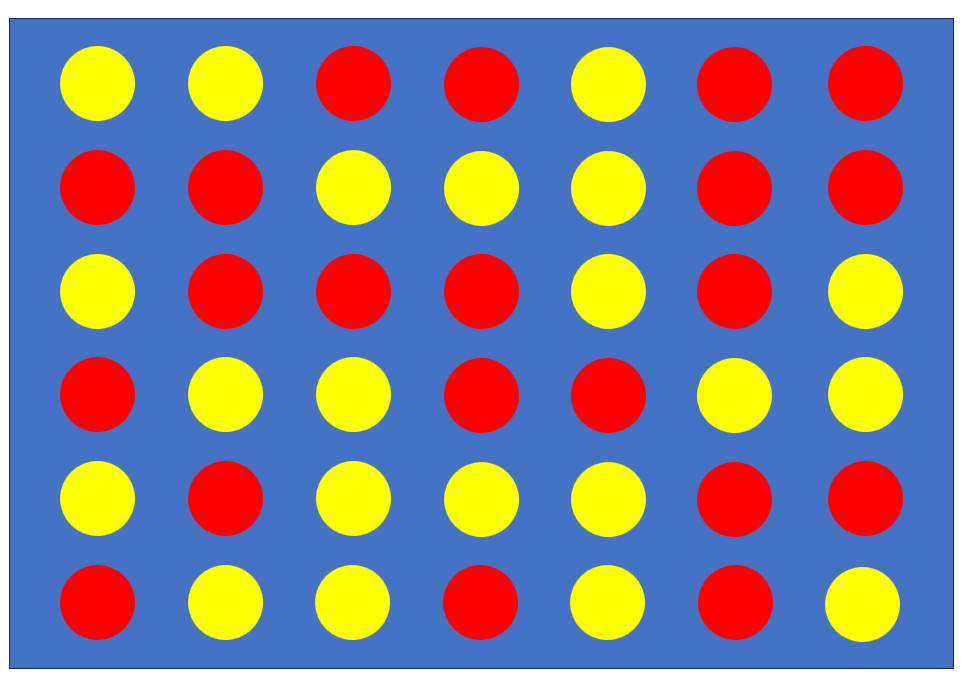
\includegraphics[width=0.8\linewidth]{images/Unentschieden}
	\caption[Unentschieden]{Unentschieden - es kam keine vierer Reihe zustande}
	\label{fig:unentschiedent}
\end{figure}
\newpage
\section{Historischer Hintergrund}
\section{Mathematische Eigenschaften des Spiels}
